\section{Introducere}

Scopul acestui proiect este acela de a implementa:
\begin{enumerate}
    \item un program care rezolvă diferite lvl pentru faimosul joc de Domino.
    \item un program care încearcă să rezolve puzzle-ul deducerii rolurilor jucătorilor din jocul „The Resistance”.
\end{enumerate} 
\newline
\subsection{Domino}

Domino este un joc celebru cu piese de domino. Doi sau mai mulți jucători trebuie să pună alternativ piesele potrivite. Câștigătorul este persoana care scapă mai întâi de toate piesele sale.
\newline
\newline
\begin{figure}[h]
    \centering
    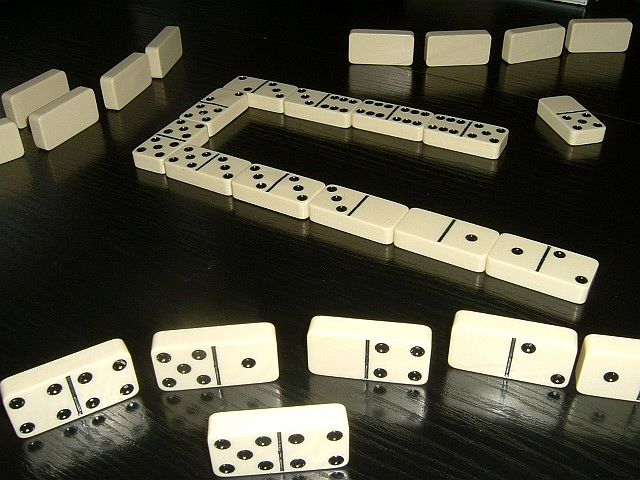
\includegraphics[width=16cm]{text/images/pic1.jpg}\\
    \caption{Domino}
\end{figure}

Avem nevoie de opt secvențe de șapte pătrate pentru piese. În total sunt 56 de pătrate. Ele reprezintă numerele de la 0 la 6. Numerele sunt reprezentate de puncte ca pe zarurile de joc. Un pătrat gol ia locul numărului 0.

\newpage
\subsection{The Resistance}

The Resistance este un joc de deducție socială care implică jucătorii care încearcă să-și dea seama cine dintre ei face parte din „Rezistență” și cine face parte din echipa „Guvernul”. Jocul este plasat într-o lume fictivă în care Rezistența încearcă să răstoarne un guvern tiranic, iar echipa de spionaj lucrează pentru a le sabota eforturile.
\newline
\newline
Fiecărui jucător i se atribuie în secret un rol la începutul jocului, iar scopul jocului este ca echipa Rezistenței să finalizeze cu succes o serie de misiuni fără a fi detectată de echipa de spionaj. Echipa de spionaj, pe de altă parte, vrea să împiedice Rezistența să reușească votând împotriva propunerilor de misiune și încercând să-și dea seama cine sunt ceilalți spioni.
\newline
\newline

\newline

\begin{figure}[h]
    \centering
    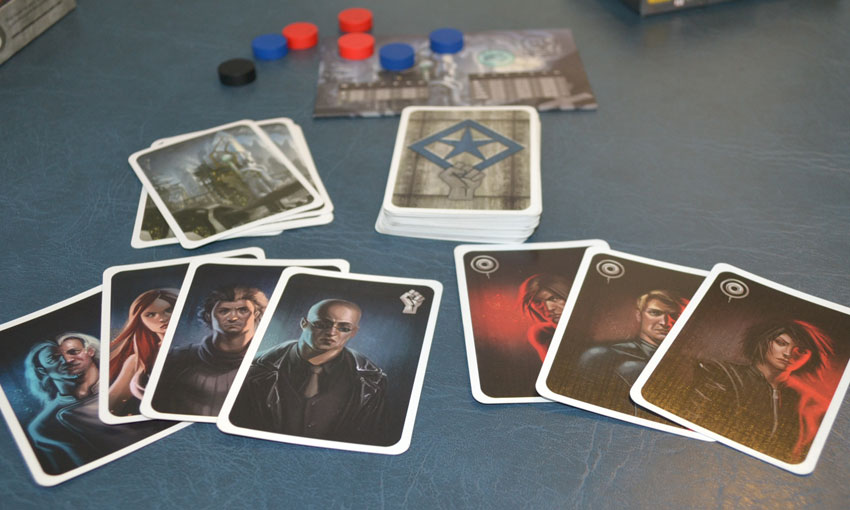
\includegraphics[width=16cm]{text/images/pic2.jpg}\\
    \caption{The Resistance Board Game}
\end{figure} \newline
\newline

\newline


\newline

\newline
Mai avem si jucători de tip Trădători, în echipa de spioni care lucrează în secret împotriva celorlalți din guvern. Acest jucător are propriile obiective secrete pe care trebuie să încerce să le ducă la bun sfârșit, încercând, de asemenea, să se îmbine cu ceilalți spioni.

Trădătorul este o răsturnare a jocului tradițional Resistance care adaugă un strat suplimentar de înșelăciune, intrigă și face și jocul mai complex.


